\section{Data Collection} \label{sec:data-collection}

For analysis, we create a dataset containing measurements from various sources about networked satellite systems. Sadly, only data from Starlink devices was included in the thesis as other satellite network systems did not have sufficient data openly available.

The data originates from RIPE Atlas, Cloudflare Radar, OONI, and N2YO. While N2YO provides data about satellites, the others hold measurement results. In the case of N2YO, the website was crawled, while the others provide API access.

The process of data collection is illustrated in Figure~\ref{fig:data-collection-process}.

\begin{figure}[h]
	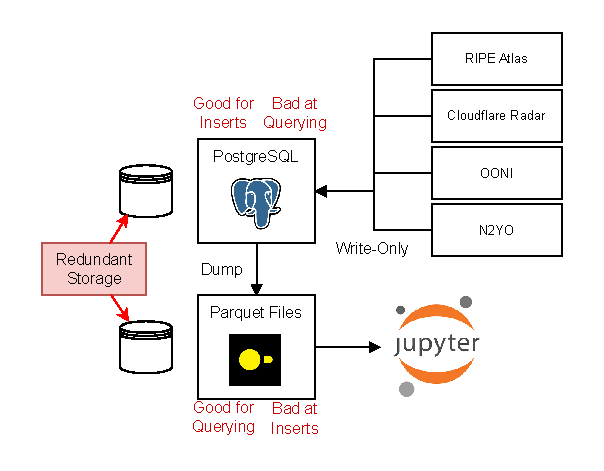
\includegraphics[width=0.7\textwidth]{./chapters/methodology/img/architecture.drawio.pdf}
	\caption{Architecture of Data Collection}
	\label{fig:data-collection-process}
\end{figure}

The data is collected from each platform and inserted into a PostgreSQL database. The database shall allow producers to quickly insert new data (i.e., new rows). Transactional databases are the best choice for that, e.g., PostgreSQL. To quickly analyze data, an analytical database is the best choice. For that purpose, Parquet files can be used. Therefore, the data from PostgreSQL is dumped into the Parquet files. This creates a redundant storage, for the sake of analysis speed.

The resulting data format is shown in Figure~\ref{fig:er-diagram}.

\begin{figure}
	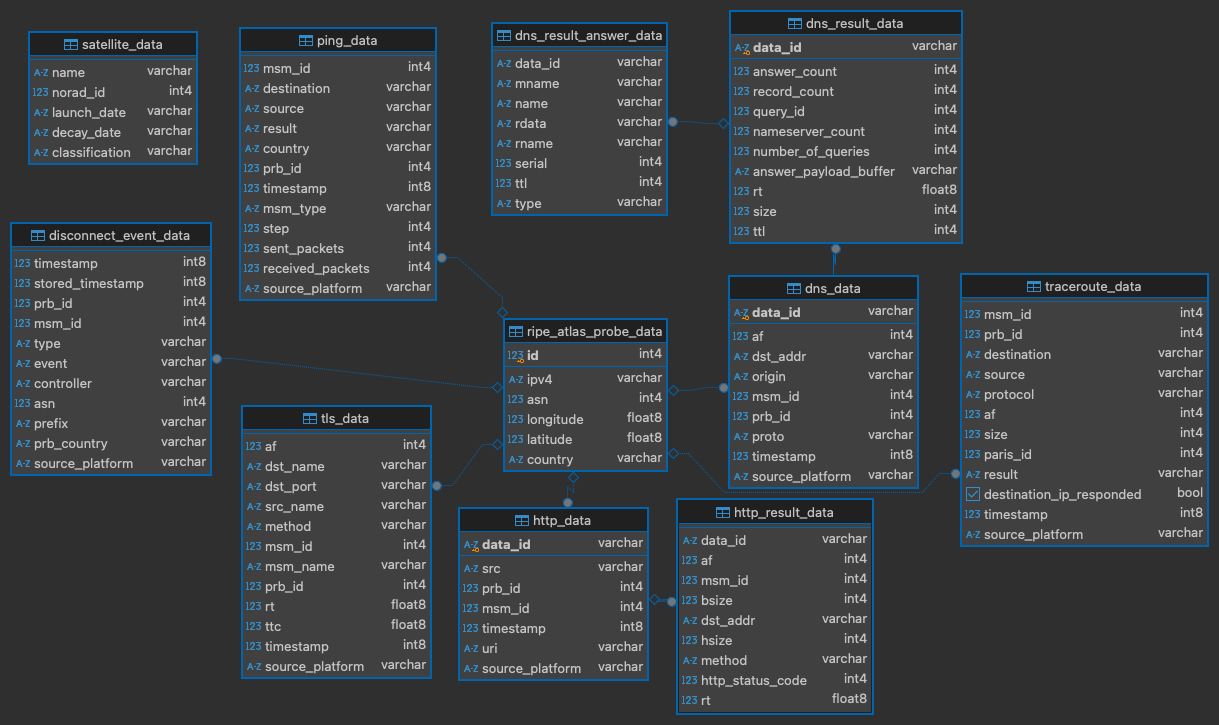
\includegraphics[width=\textwidth]{./chapters/methodology/img/er-diagram.png}
	\caption{ER Diagram on Data Schema in PostgreSQL Database.}
	\label{fig:er-diagram}
\end{figure}

The database includes Ping, Traceroute, TLS, HTTP, Disconnect Event, and DNS measurement data, as well as information about the RIPE Atlas probes and all satellites ever launched (including rocket bodies).
The whole database comprises more than 150 GB.

Additionally, the analysis uses data from IPinfo. This data is however not included in the dataset and has to be obtained from IPinfo itself.

\subsection*{RIPE Atlas Data}

RIPE Atlas offers various probes connected via networked satellite systems. At the moment of writing, all of those probes are connected via Starlink. Therefore, all the data from RIPE Atlas probes is Starlink data.

Probes are computers running the \href{https://github.com/RIPE-NCC/ripe-atlas-software-probe}{probe software from RIPE Atlas}. They are centrally connected to the RIPE Atlas servers and can be used by any person to perform measurements against them. The possible measurements are defined by the \href{https://atlas.ripe.net/docs/apis/rest-api-reference/}{RIPE Atlas REST API}.

Overall, there are 150 probes from 26 countries. Each probe performs basic measurements on a regular schedule (so-called built-in measurements). The built-in measurements are the main source of data and serve as historical record. This allows to analyze data from 2022. Even if there is Starlink data prior to 2022, it originates from very little probes and therefore will not be considered in this thesis to avoid unreliable data.
